\chapter{Empurrando Juntos} \label{cap:clusterizacao}


A democracia digital é resumida por \citeonline{penteadoencontro} como sendo o uso da Internet para consolidação da democracia.
Esse uso tem acarretado em um crescente número de discussões acerca de temas políticos, o que permitiu interessados na área analisassem 
esse fenômeno. A partir disso, foi possível observar uma polarização das mensagens trocadas nas redes sociais \cite{empurrandojuntos}.

\citeonline{empurrandojuntos} afirmou que as discussões realizadas, principalmente em redes sociais, 
acabavam refletindo sempre a opinião da maioria e que 
as pessoas estão sempre presentes em uma bolha de opinião, ou seja, as pessoas só vêem aquilo que é parecido com o que elas pensam.
Com isso, percebeu que essa polarização dificulta a participação da minoria, ou seja, aqueles que pensam diferente dos demais. 
Com suas mensagens sendo anuladas pelas mensagens trocadas pela maioria e não são apresentadas novas ideias ou pensamentos diferentes 
para quem usa essas redes sociais. 

Observando esse aspecto, o Instituto Cidade Democrática apresenta a ideia da plataforma Empurrando Juntos cujo objetivo 
é dar voz para essa minoria e tornar as discussões mais efetivas para os seus propósitos \cite{empurrandojuntos}.

A ideia é que um usuário possa criar conversas e participar de conversas criadas por outros usuários. Essa participação 
acontece de duas formas: comentando em uma conversa ou votando em um comentário de outro participante. Entende-se por voto
o ato de concordar com o comentário realizado (uma espécie de \textit{like}) ou discordar do comentário. Além disso, é permitido
que o usuário pule aquele comentário, ou seja, não atribua nenhum tipo de voto. 

Com os votos realizados, a ideia é realizar o agrupamento de pessoas que responderam de maneira parecida, ou seja, concordaram e
discordaram dos mesmos comentários. Com os grupos formados, é possível ver a convergência e divergência de opiniões e assim obter uma 
visualização mais efetiva da opinião das pessoas. A Figura \ref{fig:resumo_ej} ilustra o funcionamento básico da plataforma.

\begin{figure}[h!]
\centering
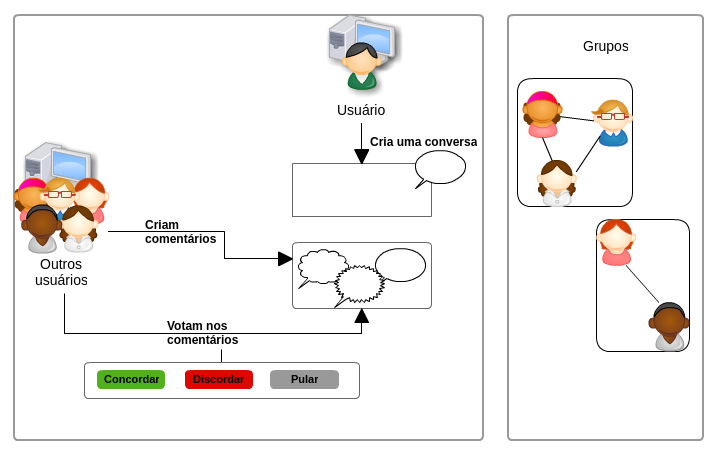
\includegraphics[scale=0.6]{figuras/resumo_ej.png}
\caption{Funcionamento do Empurrando Juntos}
\label{fig:resumo_ej}
\end{figure}



Esse agrupamento é realizado em tempo real, ou seja, conforme as pessoas vão votando são formados/modificados
os grupos. Isto é, somente se sabe que os usuários tem dados em comum, que são os votos nas conversas,
mas não há nenhum estabelecimento prévio de grupos, para que os usuários façam parte deles. 

\citeonline{han2011data} afirmam que esse processo de encontrar um modelo que possa descrever e distinguir classes de dados, ou seja, formar 
grupos, é conhecido como classificação.

\citeonline{tan2013data}, \citeonline{han2011data} e \citeonline{clustering_review} apresentam dois tipos de 
classificação: supervisionada e não supervisionada.
Na classificação supervisionada os objetos de dados são analisados a partir de rótulos de classe predefinidos nos objetos, ou seja, 
com as classes de dados previamente definidas e conhecidas. \citeonline{han2011data} chamam este tipo de dado de ``dado treinado''
(dados cujos rótulos são conhecidos), onde o modelo que o descreve é obtido a partir da análise dos rótulos.
Na classificação não supervisionada, os rótulos de classe são obtidos a partir da análise dos dados dos objetos, tão somente \cite{tan2013data}.

Uma técnica de classificação não supervisionada é a clusterização \cite{clustering_review, tan2013data}, na qual os rótulos de classes dos objetos 
podem não existir ainda e o método empregado na clusterização pode gerar rótulos para um grupo de dados do conjunto \cite{han2011data}. Considerando 
as características da plataforma Empurrando Juntos, a clusterização foi a técnica utilizada para realizar o agrupamento de pessoas.


\section{Clusterização}
A clusterização foi denominada por \citeonline{clustering_review} como uma técnica para organização ou agrupamento em \textit{clusters} 
de uma coleção de elementos que sigam padrões baseado em similaridade.
\citeonline{tan2013data} definem a análise de \textit{clusters}, ou clusterização, como a ação que agrupa objetos de dados
baseado apenas nas informações contidas nos dados do próprio objeto que permitam descrever os objetos e suas relações. Um \textit{cluster}
então pode ser visto como uma classe de objetos da qual é possível derivar regras para o grupo \cite{han2011data}.

Trata-se de uma técnica bastante utilizada em análise exploratórias, agrupamentos, 
tomada de decisão e implementações de \textit{machine learning}, como:
mineração de dados, recuperação de documentos, segmentação de imagens e padronização \cite{clustering_review}.

A técnica de clusterização pode ser dividida em alguns tipos: hierárquica ou particional; exclusiva, sobreposta ou \textit{fuzzy}; 
completa ou parcial \cite{tan2013data, clustering_review}. Na clusterização particional o agrupamento dos 
objetos de dados é realizado em simples \textit{clusters}, o que significa que pertencem apenas a um \textit{cluster} \cite{tan2013data}.

No processo de clusterização, os objetos de dados podem pertencer a um único \textit{cluster} exclusivamente ou podem
pertencer a diferentes \textit{clusters} ao mesmo tempo. 
O primeiro caso é conhecido como clusterização exclusiva e o segundo como sobreposta \cite{tan2013data}. 

% \citeonline{clustering_review} definem uma clusterização hierárquica quando ela produz uma série
% de partições aninhadas baseadas em um critério para junção ou separação dos \textit{clusters} por meio de similaridade. 
% \citeonline{tan2013data} afirmam que esse tipo de clusterização acontece quando algoritmo
% produz um resultado no qual é possível obter \textit{subclusters} e dessa forma os \textit{clusters} são aninhados
% e organizados como uma árvore, seguindo a ideia de hierarquia.

% Já o tipo \textit{fuzzy} trata da pertinência dos objetos a um grupo de forma probabilística, 
% ou em um grau de pertinência, em vez de determinar se o objeto pertence ou não àquele grupo \cite{tan2013data, clustering_review}.
% 
% Por fim, \citeonline{tan2013data} definem uma clusterização como completa quando no resultado todos os objetos estão em pelo menos um grupo. 
% Pois, na clusterização parcial alguns elementos podem ficar sem grupo caso não sejam compatíveis com algum \textit{cluster} formado.

A clusterização pode ser resumida nos passos apresentados na Figura \ref{fig:tasks_clustering}.
A seleção de características é o processo de identificação do subconjunto das características para ser utilizado na clusterização, 
e a extração de características é o uso de uma ou mais transformações das características de entrada para 
produzir mais efetivas para a clusterização. O objetivo de ambos é produzir o conjunto de objetos e dados a serem clusterizados \cite{clustering_review}.

\begin{figure}[h!]
\centering
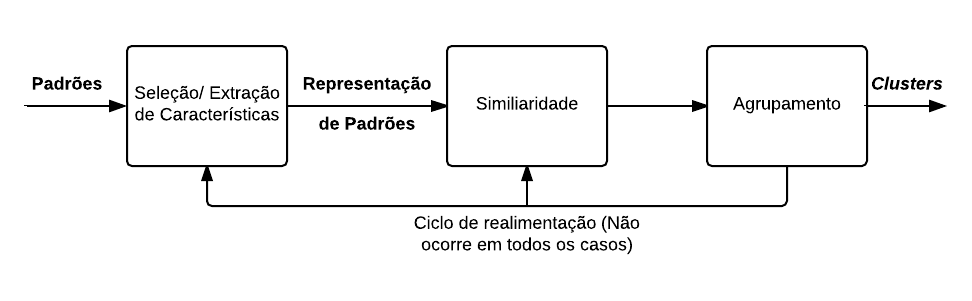
\includegraphics[scale=0.6]{figuras/tasks_clustering.png}
\caption{Passos para clusterização. Adaptado de \citeonline{clustering_review}}
\label{fig:tasks_clustering}
\end{figure}

A representação de padrões é o número de classes, número de padrões e o número, tipo e escala
das características disponíveis para a clusterização \cite{clustering_review}.

A similaridade é medida, em geral, por uma função de distância entre um par de objetos. Além disso, utiliza-se também
o conceito inverso de dissimilaridade para calcular o quanto objetos são diferentes. Essa função de distância pode variar de acordo 
com o contexto da aplicação e tipo dos dados. 

E por fim, o agrupamento pode ser realizado com uso de inúmeras técnicas e algoritmos diferentes \cite{clustering_review}.
Os objetos são agrupados (ou "clusterizados") buscando maximizar a similaridade intraclasse e minimizar a similaridade interclasse.
Em outras palavras, o objetivo é formar \textit{clusters} cujos elementos tenham alta similaridade entre si em um mesmo \textit{cluster} 
e baixa similaridade a elementos de outros \textit{clusters} \cite{han2011data}.

Apesar de parecer lógico e simples querer maximizar a similaridade intraclasse e minimizar a similaridade interclasse entre um conjunto de dados, 
\citeonline{tan2013data} exemplificam o quão difícil esta tarefa pode ser na Figura \ref{fig:clusters_difficulty}, onde temos um conjunto
de pontos (a) que pode ser agrupado de formas diferentes gerando quantidades diferentes de \textit{clusters} (b, c, d).

\begin{figure}[ht!]
\centering
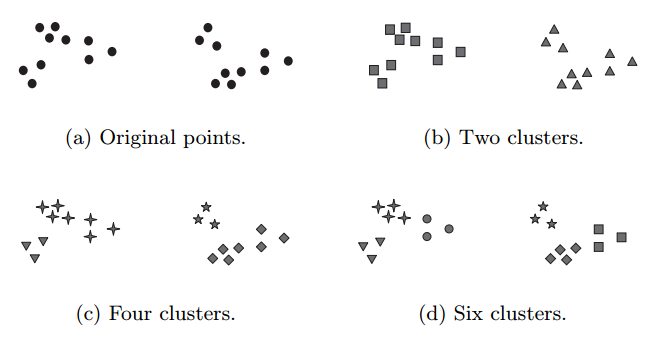
\includegraphics[scale=0.4]{figuras/clusters_difficulty.png}
\caption{Formas de se agrupar o mesmo conjunto de dados. Fonte: \cite{tan2013data}}
\label{fig:clusters_difficulty}
\end{figure}

Por isso para a construção de um algoritmo de clusterização deve-se definir, além do algoritmo principal a ser utilizado, as funções
de cálculo de similaridade e dissimilaridade para delimitação dos \textit{clusters}.

\vfill
\pagebreak

\section{Módulo de clusterização do Empurrando Juntos}

A clusterização implementada no Empurrando Juntos é baseada em um algoritmo bastante popular denominado k-Means. O k-Means é um
algoritmo particional e de clusterização exclusiva que forma k clusters a partir de k centróides, onde k é um número definido na aplicação 
\cite{clustering_review, tan2013data}. Um centróide é entendido, conceitualmente, como um ponto central \cite{han2011data}.

O algoritmo foi descrito por \citeonline{tan2013data} e \citeonline{han2011data} da seguinte forma:


\lstset{language=HTML, numbers=left, stepnumber=1}
\begin{lstlisting}
Escolha K pontos, dentro do conjunto de pontos a serem clusterizados ou não, como centróides iniciais
Repita:
  Forme K clusters de acordo com a menor distância dos pontos ao centróide, movendo os pontos para cada cluster.
  Recalcule o centróide de cada cluster baseado nos pontos do cluster.
Até que os centróides não mudem.
\end{lstlisting}

Nota-se que o número de centróides escolhidos determina a quantidade de clusters no final do processamento.
Para o cálculo da distância entre os pontos é utilizado um cálculo conhecido como distância Euclidiana, 
dado pela fórmula \ref{eq:euclidiana} \cite{clustering_review, tan2013data, han2011data}.

\begin{equation} \label{eq:euclidiana}
  d_{2}(x_i, x_j) = (\sum_{k=1}^{d} (x_{i,k} - x_{j,k})^2)^{1/2}
\end{equation}

A variação dentro do cluster é calculada pela fórmula \ref{eq:variacao}, na qual a 
função \textit{dist} representa a distância Euclidiana entre um ponto do
cluster e seu centróide. Ou seja, a variação é a soma dos quadrados
das distâncias de todos os pontos do cluster.

\begin{equation} \label{eq:variacao}
  E = \sum_{i=1}^{k} \sum_{p \epsilon C_{i}} dist(p, c_i)^2
\end{equation}

Na Figura \ref{fig:iteracoes_kmeans} é apresentada um exemplo das iterações utilizando o algoritmo.

\begin{figure}[h!]
\centering
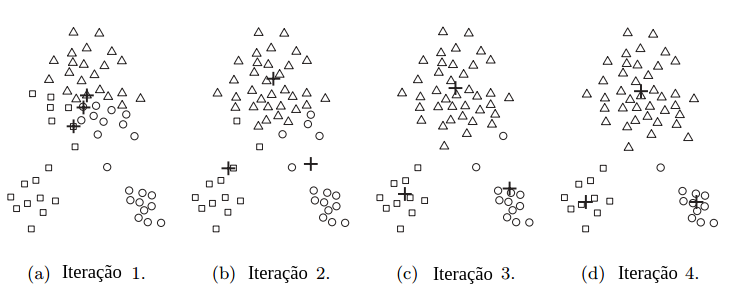
\includegraphics[scale=0.6]{figuras/iteracoes_kmeans.png}
\caption{Iterações de clusterização utilizando k-Means. Adaptado de \citeonline{tan2013data}}
\label{fig:iteracoes_kmeans}
\end{figure}

No Empurrando Juntos a entrada para os \textit{clusters} é a combinação entre participante,  
comentário e o voto. Essa combinação gera uma entrada de N dimensões para N comentários.
Frequentemente antes de medir a similaridade entre os objetos é necessário
reduzir a dimensionalidade, isso acontece, pois para espaços de alta dimensão as distâncias euclidianas
tendem a inflar e reduzir a dimensionalidade pode aliviar este problema e reduzir o tempo de cálculo.
Um dos métodos mais utilizados para realizar essa redução é a Análise de 
Componentes Principais (PCA, do inglês) \cite{han2011data, sklearn}.


\citeonline{han2011data} afirmam que o PCA cria K vetores ortogonais que possuem o mesmo significado que o conjunto
de vetores inicial, porém trata-se de um conjunto menor. Para aplicação desse método são realizados basicamente quatro procedimentos.

\begin{enumerate}
 \item Normalizar os dados de entrada, para que eles estejam dentro da mesma variação;
 \item Computar k vetores ortonormais, ou seja, vetores de magnitude 1, nos quais cada ponto é perpendicular aos outros;
  \subitem Esses vetores são chamados de componentes principais.
 \item Ordenar decrescentemente os componentes principais pela significância;
 \item Remover os componentes ``fracos'', ou seja, aqueles com pouca variância.
\end{enumerate}

No final dos quatro procedimentos, os componentes principais restantes são uma boa aproximação dos dados originais \cite{han2011data}.

Definir previamente o valor de K, ou seja, o número de \textit{clusters} é considerada uma das desvantagens desse algoritmo. Todavia,
é possível contornar essa desvantagem escolhendo um intervalo de valores para execução do algoritmo e em seguida aplicar
uma técnica analítica para definir o melhor valor \cite{han2011data}. Uma técnica analítica para a definição do melhor valor para K utilizada pelo Empurrando Juntos
é conhecida como Coeficiente de silhueta \cite{sklearn}.

Essa técnica tem por objetivo combinar a avaliação de coesão e separação dos clusters por meio do cálculo de um coeficiente (o de silhueta) que 
varia de -1 a 1 e é dado pela fórmula \ref{eq:coeficiente} \cite{tan2013data}.

\begin{equation} \label{eq:coeficiente}
  s_{i} = \frac{(b_{i} - a_{i})}{max(a_{i}, b_{i})} \mbox{, onde:}
\end{equation}

{\addtolength{\leftskip}{8mm}
    i é o objeto do \textit{cluster} que está sendo analisado
    
    $a_{i}$ é a média da distância entre o objeto e todos os objetos do seu \textit{cluster}
    
    $b_{i}$ é o valor mínimo entre o objeto e os demais \textit{clusters}. 
    
	  \footnotesize \indent \indent A distância entre o objeto e outro \textit{cluster} é média da distância entre o objeto \\ \indent \indent e todos os objetos do outro \textit{cluster}.
}

Um coeficiente negativo representa que o elemento está no \textit{cluster} errado, pois isso significa que a distância entre o objeto e outro \textit{cluster} 
é menor que a distância entre o objeto e os objetos de seu \textit{cluster}. O valor ``zero'' representa que o elemento está próximo da ``borda'' do \textit{cluster}, ou seja,
as distância entre o objeto e outros \textit{clusters} e entre o objeto e os objetos de seu \textit{cluster} é a mesma. E por fim, quanto mais próximo do valor 1, melhor
está a distribuição dos \textit{clusters}, pois significa que o valor de $a_i$ é menor que o valor de $b_i$.

Dessa forma, com a escolha de um intervalo de valores para K, como sugerido por \citeonline{han2011data} e \citeonline{sklearn}, permite testar os valores para o coeficiente
de silhueta e escolher o melhor valor de K dentro do intervalo. 


Na Figura \ref{fig:exemplo_silhueta} é apresentado um exemplo visual de \textit{clusters} com diferentes valores
de K e seus coeficientes de silhueta.

\begin{figure}[bt!]
\centering
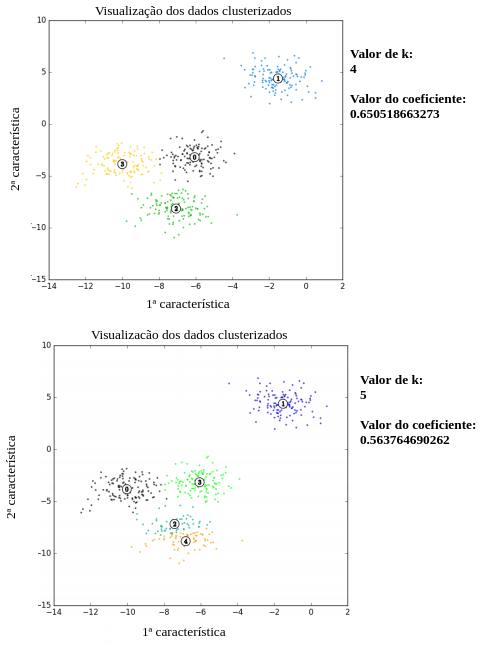
\includegraphics[scale=1]{figuras/exemplo_silhueta.png}
\caption{Formação de \textit{clusters} utilizando K-means e seus coeficientes de silhueta. Adaptado de \citeonline{sklearn}}
\label{fig:exemplo_silhueta}
\end{figure}

\vfill
\pagebreak

Os métodos e técnicas apresentados fazem parte do algoritmo implementado no módulo de clusterização da plataforma 
e possuem um objetivo específico. O fluxo seguido pelo algoritmo de clusterização do Empurrando Juntos pode ser resumido de acordo comm
a Figura \ref{fig:resumo_clusterizao_ej} que apresenta um esquemático desse módulo.

\begin{figure}[h!]
\centering
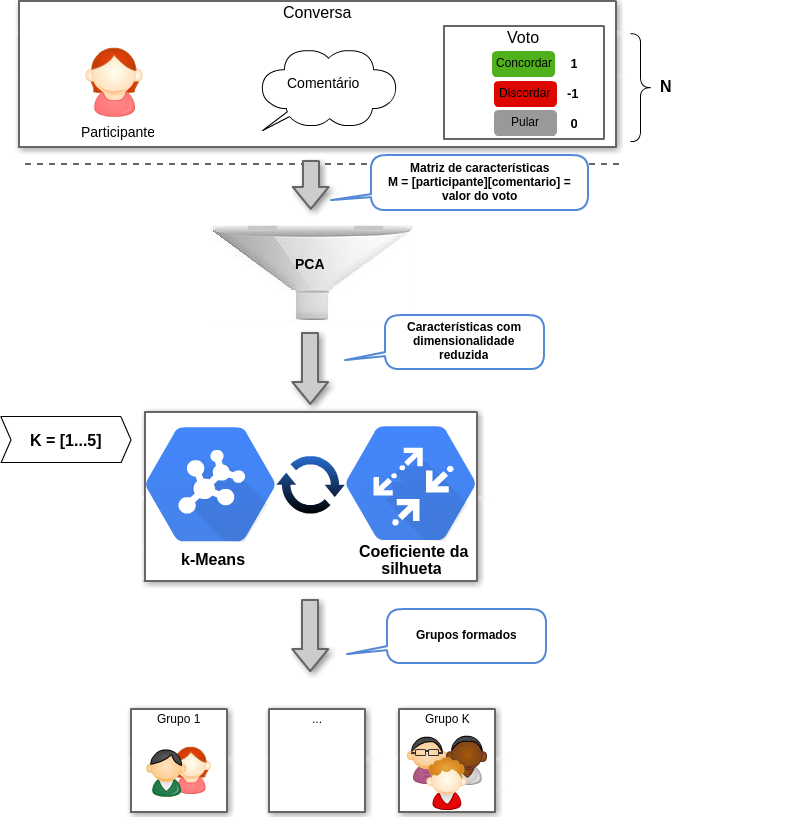
\includegraphics[scale=0.7]{figuras/resumo_clusterizao_ej.png}
\caption{Fluxo de clusterização do Empurrando Juntos}
\label{fig:resumo_clusterizao_ej}
\end{figure}

%%%fazer um gancho para a API

